\begin{figure*}
% \vspace{-0.7cm}
    \centering
    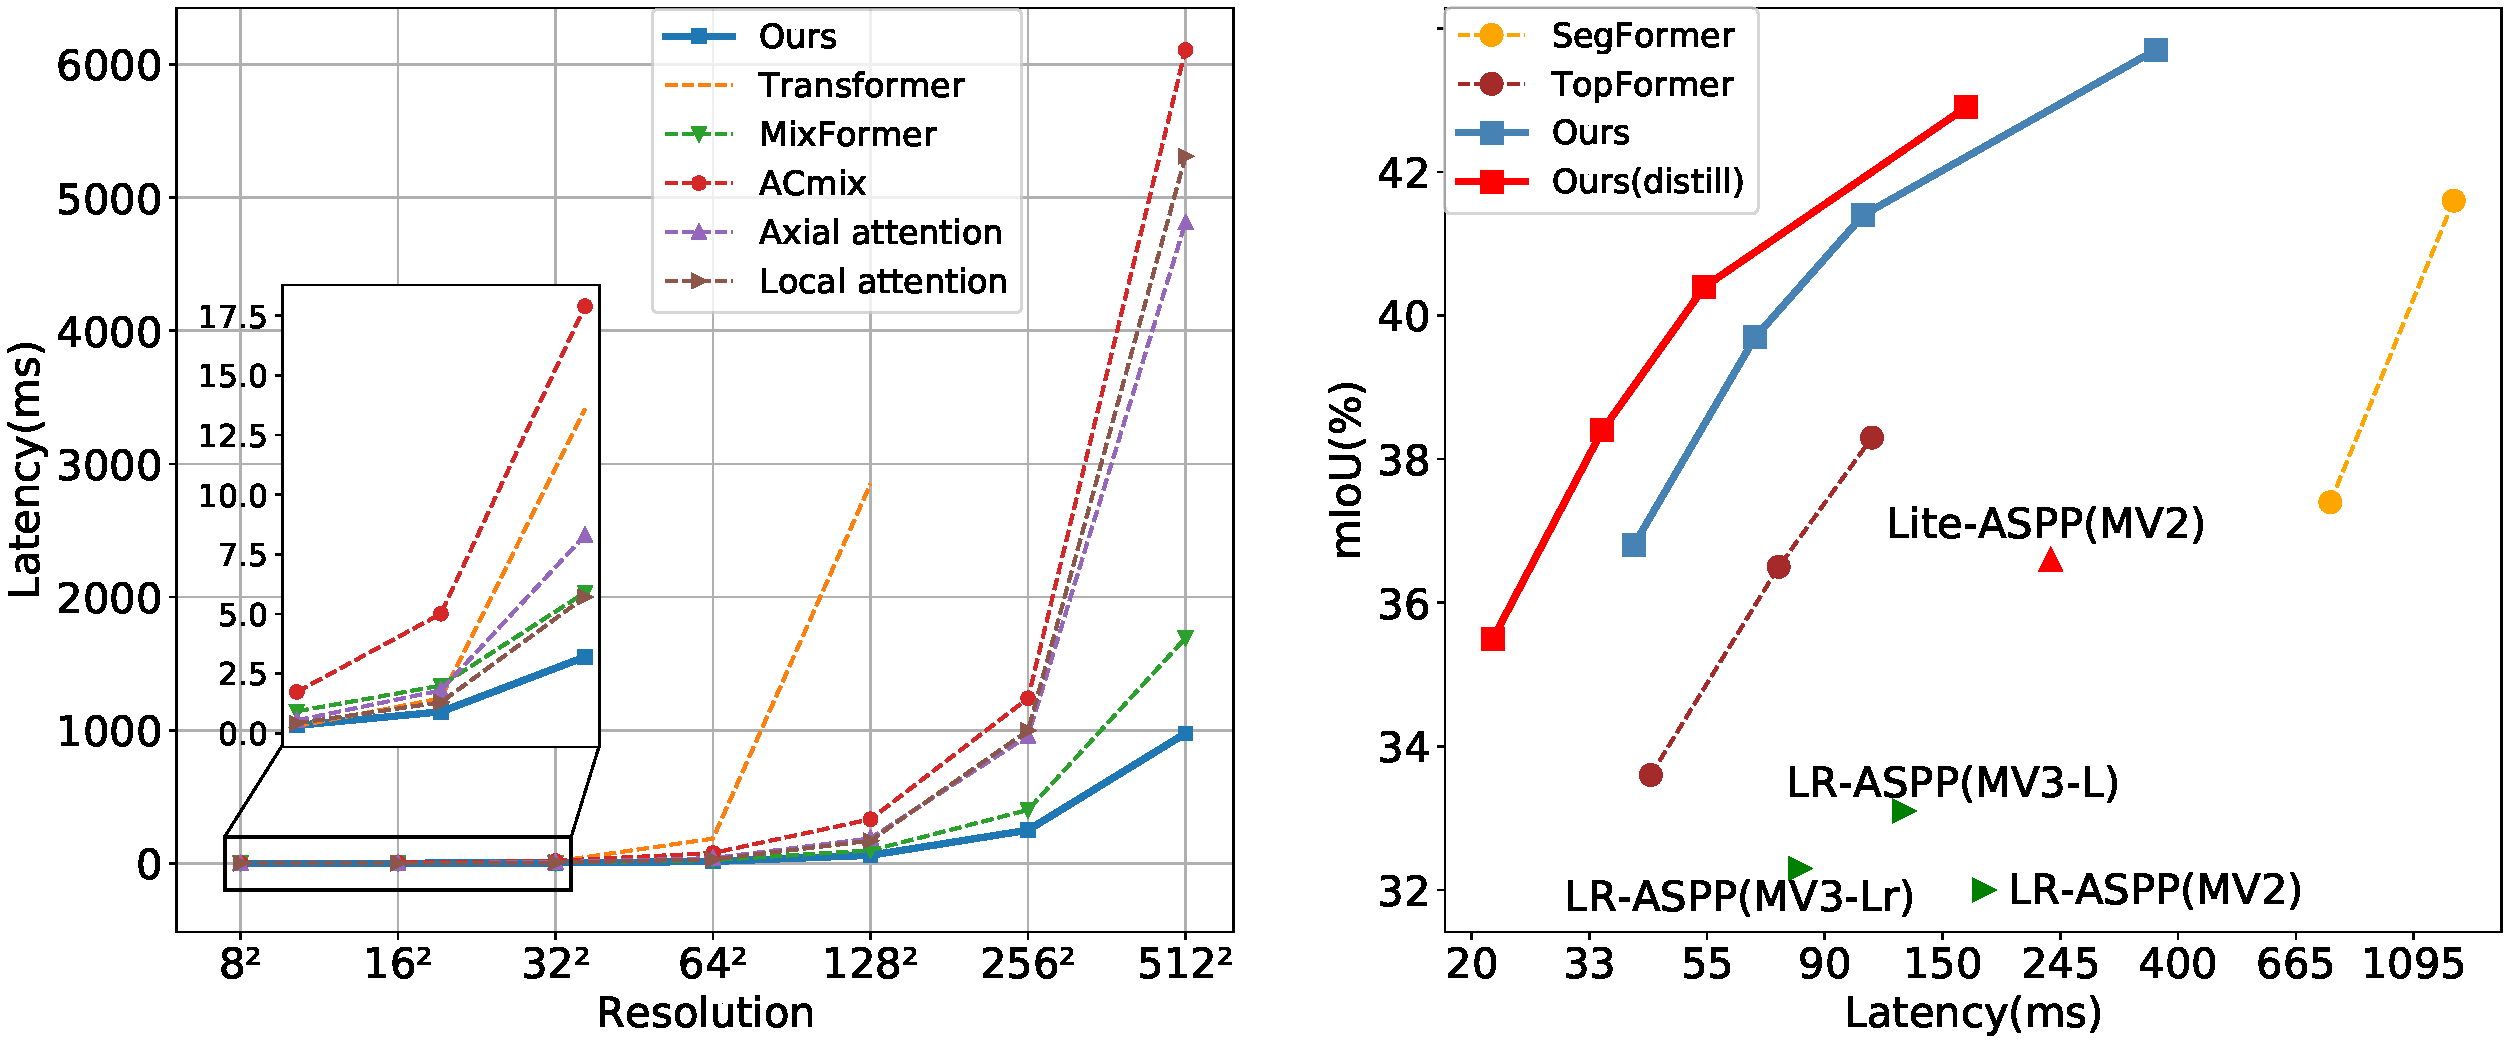
\includegraphics[width=\linewidth]{latency_vs_pixel2.pdf}
    \caption{\textit{\textbf{Left}}: 
    Latency comparison with Transformer~\cite{vaswani2017attention}, MixFormer~\cite{chen2022mixformer}, ACmix~\cite{pan2022integration}, 
    Axial attention~\cite{ho2019axial} and 
    local attention~\cite{luong2015effective}. 
    It is measured with a single module of channel dimension 64 on a Qualcomm Snapdragon 865 processor. 
    \textit{\textbf{Right}}: 
    The mIoU versus latency on the ADE20K \textit{val} set. 
    MV2 means MobileNetV2~\cite{sandler2018mobilenetv2}. 
    MV3-L means MobileNetV3-Large~\cite{howard2019searching}. 
    MV3-Lr denotes MobileNetV3-Large-reduce~\cite{howard2019searching}. 
    The latency is measured on a single Qualcomm Snapdragon 865, and only an ARM CPU core is used for speed testing. No other means of acceleration, e.g., GPU or quantification, is used. For figure \textit{Right}, the input size is 512×512. SeaFormer achieves superior trade-off between mIoU and latency.}
    \label{fig:latency_comp}
% \vspace{-0.2cm}
\end{figure*}